\begin{figure}[htbp]
\centering
\begin{tikzpicture}[x=1cm,y=1cm]
\node[anchor=south west,inner sep=0] at (0,0) {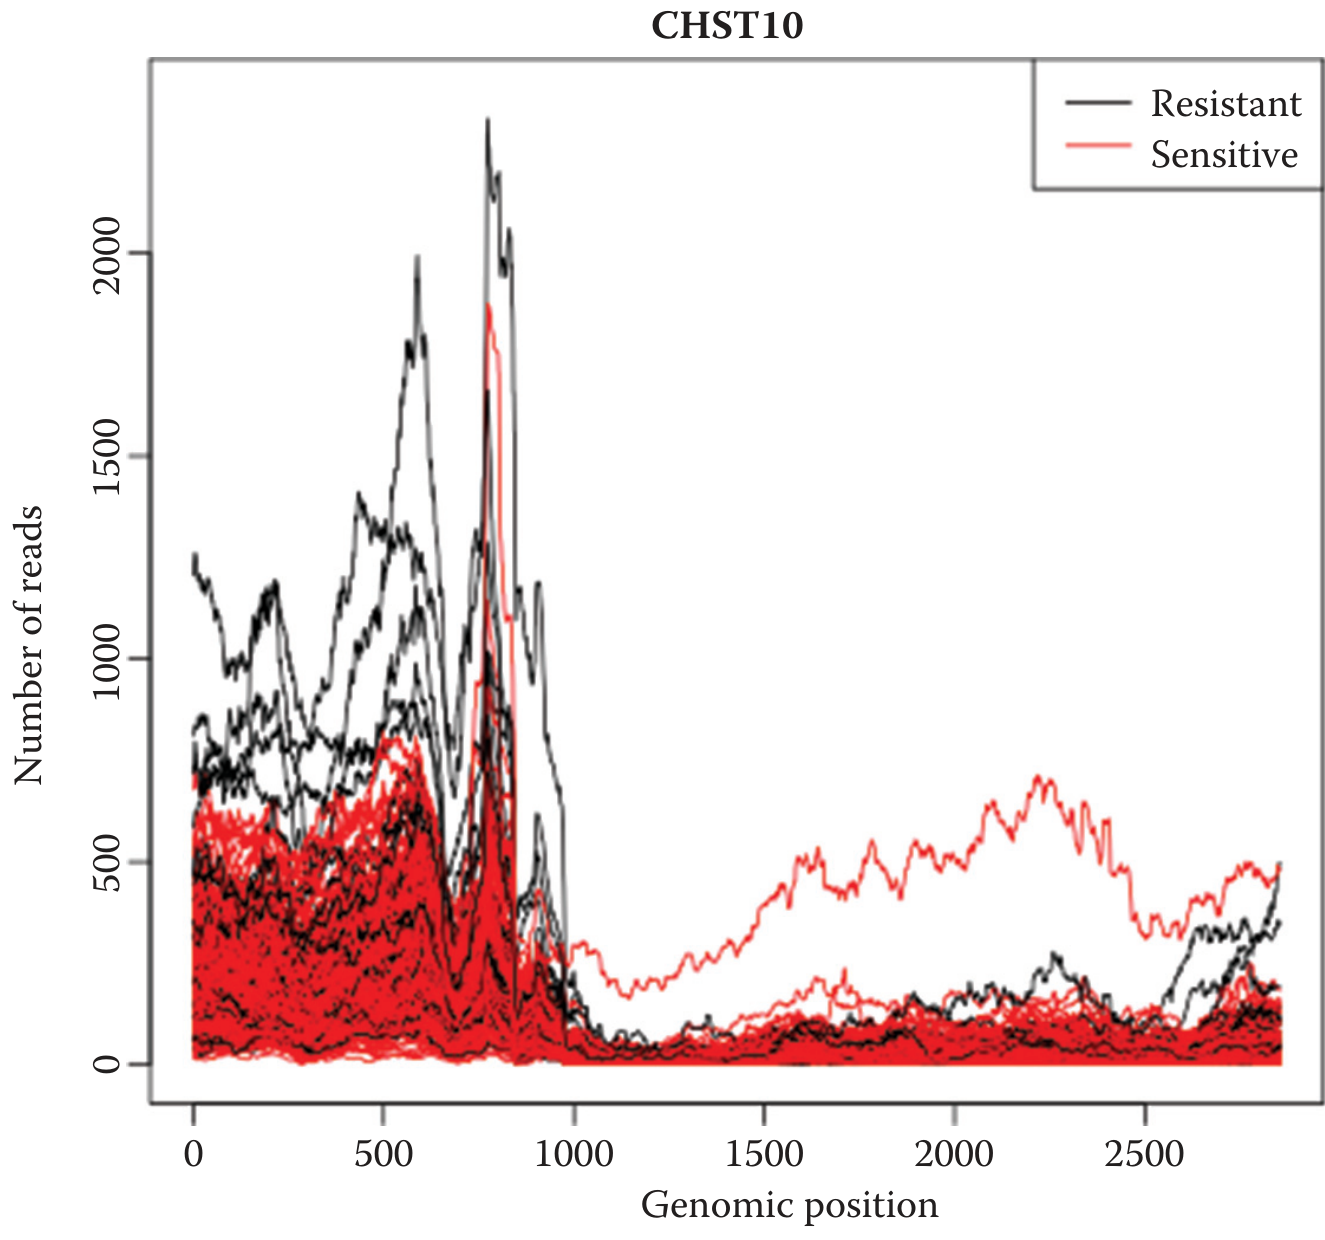
\includegraphics[width=11.3cm]{figures/ch04a_fig13_data.png}};
\fill[white] (5.4362,0.0866) rectangle (8.0365,0.4778);
\node[inner sep=0pt,fill=white,rotate=0,font=\fontsize{8}{8}\selectfont] at (6.7364,0.2822) {基因组位置};
\fill[white] (0.0703,3.8479) rectangle (0.4615,6.2947);
\node[inner sep=0pt,fill=white,rotate=90,font=\fontsize{8}{8}\selectfont] at (0.2659,5.0713) {读段数};
\fill[white] (9.7874,9.4753) rectangle (11.1317,9.8664);
\node[inner sep=0pt,fill=white,rotate=0,font=\fontsize{8}{8}\selectfont] at (10.4595,9.6708) {耐药};
\fill[white] (9.7874,9.0405) rectangle (11.0989,9.4316);
\node[inner sep=0pt,fill=white,rotate=0,font=\fontsize{8}{8}\selectfont] at (10.4432,9.2361) {敏感};
\end{tikzpicture}
\origfig{13}{TCGA 卵巢癌数据集中基因 CHST10 的表达谱。}
\label{fig:ch04a-13}
\end{figure}
